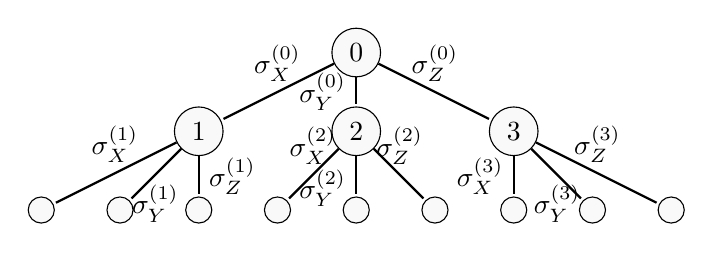
\begin{tikzpicture}[
    shorten > = 1pt,
node distance = 3cm and 4cm,
    el/.style = {inner sep=2pt, align=left, sloped},
every label/.append style = {font=\tiny}
                    ]
\node[shape=circle,draw=black,fill=gray!5] (0) at (4,2) {0}; 
\node[shape=circle,draw=black,fill=gray!5] (1) at (2,1) {1};
\node[shape=circle,draw=black,fill=gray!5] (2) at (4,1) {2};
\node[shape=circle,draw=black,fill=gray!5] (3) at (6,1) {3};
\node[shape=circle,draw=black,fill=gray!5] (4) at (0,0) {};
\node[shape=circle,draw=black,fill=gray!5] (5) at (1,0) {};
\node[shape=circle,draw=black,fill=gray!5] (6) at (2,0) {};
\node[shape=circle,draw=black,fill=gray!5] (7) at (3,0) {};
\node[shape=circle,draw=black,fill=gray!5] (8) at (4,0) {}; 
\node[shape=circle,draw=black,fill=gray!5] (9) at (5,0) {}; 
\node[shape=circle,draw=black,fill=gray!5] (10) at (6,0) {}; 
\node[shape=circle,draw=black,fill=gray!5] (11) at (7,0) {}; 
\node[shape=circle,draw=black,fill=gray!5] (12) at (8,0) {}; 



\path [-] (0) edge[color=black,thick] node[pos=0.5, above] {$\sigma^{(0)}_X$} (1);
\path [-] (0) edge[color=black,thick] node[pos=0.5, left]  {$\sigma^{(0)}_Y$} (2);
\path [-] (0) edge[color=black,thick] node[pos=0.5, above]  {$\sigma^{(0)}_Z$} (3);
\path [-] (1) edge[color=black,thick] node[pos=0.5, above] {$\sigma^{(1)}_X$} (4);
\path [-] (1) edge[color=black,thick] node[pos=0.5, below] {$\sigma^{(1)}_Y $} (5);
\path [-] (1) edge[color=black,thick] node[pos=0.5, right] {$\sigma^{(1)}_Z $} (6);
\path [-] (2) edge[color=black,thick] node[pos=0.5, above] {$\sigma^{(2)}_X$} (7);
\path [-] (2) edge[color=black,thick] node[pos=0.8, left] {$\sigma^{(2)}_Y $} (8);
\path [-] (2) edge[color=black,thick] node[pos=0.5, above] {$\sigma^{(2)}_Z $} (9);
\path [-] (3) edge[color=black,thick] node[pos=0.5, left] {$\sigma^{(3)}_X$} (10);
\path [-] (3) edge[color=black,thick] node[pos=0.5, below] {$\sigma^{(3)}_Y$} (11);
\path [-] (3) edge[color=black,thick] node[pos=0.5, above] {$\sigma^{(3)}_Z$}(12);

\end{tikzpicture}